% Supplementary material for main.tex (figures made by Python/paper_si_*.py, style Python/paper_style.py)
\documentclass[12pt]{article}
\usepackage[margin=25mm]{geometry}
\usepackage{amsmath,amssymb}
\usepackage{bm}
\usepackage{graphicx}
\graphicspath{{figures/}}
\usepackage{siunitx}
\usepackage[authoryear]{natbib}
\usepackage{xr-hyper}
\usepackage[hidelinks]{hyperref}
% Labels of the paper (build main.tex first, into build/)
\externaldocument[M-]{build/main}
\renewcommand{\thefigure}{S\arabic{figure}}
\renewcommand{\thetable}{S\arabic{table}}
\renewcommand{\thesection}{S\arabic{section}}
\renewcommand{\theequation}{S\arabic{equation}}
\usepackage{booktabs}
\usepackage{adjustbox}

\title{Supplementary material for ``Working-fluid-free measurement of particle number concentration
and water vapor from the laser-extinction curve of an expansion cloud by simulation-based inference''}
\author{Nobuhiro Moteki}
\date{}

\begin{document}
\maketitle

\section{Parts and cost}
\label{sec:s-parts}
Table~\ref{tab:s_parts} lists the parts of the instrument (Sect.~\ref{M-sec:instrument} of the paper). The
pressure sensor, the data acquisition device and the laptop computer account for about two thirds of the
cost, and each of them can be replaced by a much cheaper part. The analysis of a cycle takes about
0.1\,s (Sect.~\ref{M-sec:npe} of the paper), so that a single-board computer with an analog-to-digital
converter
should suffice. A cheaper pressure sensor can be used if its response time is about 10\,ms or
shorter, like that of the present one (Sect.~\ref{sec:s-pform}).

\begin{table}[!htbp]
\centering
\caption{Parts and approximate cost of the instrument (prices of 2026, mostly excluding tax,
rounded). The total corresponds to about US\$4700.}
\label{tab:s_parts}
\begin{adjustbox}{max width=\textwidth}\small% Parts and approximate cost (survey of 2026, retail or list prices, mostly excluding tax; rounded).
% Sources in Docs/costs/parts_current.md; re-check before submission.
\begin{tabular}{llrr}
\toprule
Component & Model & Qty & Approx. cost (JPY) \\
\midrule
Round-bottom flask, borosilicate glass, 3000\,mL & HARIO MF-3L & 1 & 18\,000 \\
Silicone stopper & AS ONE No.~13 & 1 & 600 \\
Motorized ball valve, DC 24\,V & KITZ ED24 series & 2 & 64\,000 \\
Pump (free-piston) & Nitto Kohki VP0940 & 1 & 60\,000 \\
Laser diode module, 670\,nm, 3\,mW & Global Laser LDL175 or equivalent & 1 & 41\,000 \\
Si photodiode, 3.6\,mm $\times$ 3.6\,mm & Hamamatsu S1223-01 & 1 & 3\,400 \\
Barometric pressure sensor, 0--1380\,hPa (0--20\,psia) & Setra 276 & 1 & 140\,000 \\
Thin-film thermistor, 10\,k$\Omega$ & -- & 1 & 500 \\
Data acquisition, 16 bit & NI USB-6210 & 1 & 180\,000 \\
Conductive silicone tubing, i.d. 4.8\,mm$^{a}$ & TSI 3001788 & 3\,m & 26\,000 \\
Tygon tubing, i.d. 2\,mm & -- & 0.6\,m & 6\,400 \\
24\,V power supply, relay board, photodiode amplifier, stainless tubes & -- & -- & 10\,000 \\
Laptop computer (6-core CPU, 16\,GB RAM) & Dell Pro 16 & 1 & 150\,000 \\
\midrule
Total & & & about 700\,000 \\
\bottomrule
\multicolumn{4}{l}{\footnotesize $^{a}$ Sold in rolls; the cost of the length used is given.}\\
\end{tabular}
\end{adjustbox}
\end{table}

\section{Thermodynamics, optical path and numerics of the forward model}
\label{sec:s-thermo}
The air in the optically probed core of the sealed flask is treated as a closed, adiabatic system of
unit mass of dry air with water vapor $q_v$ and liquid water $q_l$, $q_v + q_l = q_w$ = const. Its
volume is $v = (R_d + q_v R_v)\,T/p$ (ideal gases at the common pressure $p$, liquid volume
neglected). With no heat exchange and only the work of expansion, the first law gives
$du = -p\,dv$, i.e.\ for the enthalpy $h = u + pv$,
\begin{equation}
dh = v\,dp .
\label{eq:s-first-law}
\end{equation}
This holds whether or not the condensation proceeds in equilibrium, since the vapor, the droplets and
the air exchange heat only with each other. The enthalpy is
$h = c_{pd}T + q_v h_v(T) + q_l h_l(T)$, with $dh_v/dT = c_{pv}$, $dh_l/dT = c_l$ and
$h_v - h_l = l_v$, so that, with $dq_l = -dq_v$,
\begin{equation}
dh = \left(c_{pd} + q_v c_{pv} + q_l c_l\right) dT + l_v\,dq_v .
\end{equation}
Combining the two equations and dividing by $dt$ gives Eq.~(\ref{M-eq:temperature}) of the paper,
\begin{equation}
c_p \frac{dT}{dt} = -l_v \frac{dq_v}{dt} + T\,(R_d + q_v R_v)\,\frac{1}{p}\frac{dp}{dt} .
\end{equation}
Without condensation it reduces to the dry adiabat of moist air. The latent heating is written with
$dq_v/dt$ and the total pressure $p$, so no approximation of the partial pressure of dry air is needed.

The vapor pressure follows from Dalton's law, $e = q_v p/(\varepsilon + q_v)$ with
$\varepsilon = R_d/R_v = 0.622$, and the saturation vapor pressure over a plane water surface from the
Clausius--Clapeyron equation \citep[Eq.~4-83]{pruppacher1997microphysics} integrated with a constant
latent heat, $e_s(T) = A\exp(-B/T)$ with $A = \SI{2.5368e11}{\pascal}$ and $B = \SI{5420.5}{\kelvin}$
($\approx l_v/R_v$). It agrees with the formulation of \citet{murphy2005review} within 1\,\% between
260 and 290\,K, which covers the cloud formation. At 300\,K the difference is about 2\,\%. The constants
used are
$R_d = \SI{287.04}{\joule\per\kilogram\per\kelvin}$, $R_v = \SI{461.5}{\joule\per\kilogram\per\kelvin}$,
$c_{pd} = \SI{1005}{\joule\per\kilogram\per\kelvin}$, $c_{pv} = \SI{1850}{\joule\per\kilogram\per\kelvin}$,
$c_l = \SI{4218}{\joule\per\kilogram\per\kelvin}$, $\rho_l = \SI{1000}{\kilogram\per\cubic\meter}$ and
$l_v = \SI{2.501e6}{\joule\per\kilogram}$ (its value at 0\,$^\circ$C, held constant). This neglects the
temperature dependence
$dl_v/dT = c_{pv} - c_l$ implied by the enthalpies above, which changes $l_v$ by at most about 1\,\%
between $-11$ and $+6$\,$^\circ$C, where the cloud forms.
The surface tension is $\sigma_w = 0.0761 - 1.55\times10^{-4}\,(T - 273.15\,\mathrm{K})$\,N\,m$^{-1}$.
The density of the air is $\rho_a = p/(R_d T)$, and the number concentration per unit volume reported in
the paper is $N\,p_\mathrm{ini}/(R_d T_\mathrm{ini})$, the same conversion as used for the comparison
with the CPC.

Heat conduction from the wall is neglected in the model, which describes the adiabatic core of the
flask. The wall stays at the initial temperature, while the expanding gas has cooled by 20--30\,K
at the time of the inference window. By conduction alone, the gas at a distance $\delta$ from the wall is
warmed by the fraction $\mathrm{erfc}[\delta/(2\sqrt{D_\mathrm{th} t})]$ of this difference, with the thermal
diffusivity of air $D_\mathrm{th} \approx \SI{2.4e-5}{\square\meter\per\second}$ at the reduced pressure.
A tenth
of the difference reaches $\delta \approx 1.2$--1.5\,cm at the start of the inference window
(1.1--1.6\,s after $t_0$) and 1.6--1.9\,cm at its end (2.1--2.6\,s after $t_0$; 5--95\,\% of the
cycles). If the cloud
vanished wherever the gas had been warmed by this much, the optical path through the cloud (inner
diameter about 0.197\,m) would shorten from about 0.17\,m at the start of the window to about 0.16\,m at
its end, against the 0.18\,m assumed in the paper.

This was tested against the recorded curves (Table~\ref{tab:s_path}). For the 104 cycles of
Sect.~\ref{sec:s-nuisance}, $\log_{10}N$ was fitted as there ($q_w$ fixed at the hygrometer value, reference
nuisance parameters) with constant paths of 0.16--0.19\,m and with a path
that shrinks in time as above, $L(t) = \min[0.18\,\mathrm{m},\, 0.197\,\mathrm{m} - 2b\sqrt{t}]$ with
$b = 2c\sqrt{D_\mathrm{th}}$ (m\,s$^{-1/2}$) and $\mathrm{erfc}(c) = 0.1$ (or half of this $b$).
A path of 0.19\,m fits the curves worse than 0.18\,m.
Paths of 0.16 and 0.17\,m and the shrinking path give a slightly lower median misfit than 0.18\,m,
but none fits better in a clear majority of the cycles (44--59\,\%). The differences are small.
With half of $b$ the path stays at 0.18\,m through nearly all of the window, so that it gives the
same $N$ as 0.18\,m.
After the window ($t_\mathrm{s}$ + 1.2--1.5\,s), the measured Tr lies above the curve simulated with 0.18\,m
by
a median of $9\times10^{-3}$ at $N$ below 1100\,cm$^{-3}$ and $4\times10^{-3}$ above 2100\,cm$^{-3}$.
The shrinking path lowers this residual by about $3\times10^{-3}$ at low $N$ and by about
$10\times10^{-3}$ at high $N$, so that it overshoots at high $N$. Shorter constant paths act in the
same way.
The curves thus allow a thicker cloud-free layer or one that thickens by conduction. Such a layer
does not explain why the measured Tr stops falling, which happens mostly at low $N$. A path of 0.17\,m
would make $N$ about 8\,\% higher (Sect.~\ref{M-sec:budget} of the paper).

Figure~\ref{fig:s_residuals} shows the residual of the forward model at the posterior median (reference
nuisance parameters) for every fifth validated cycle (623 cycles). The script is
\texttt{Python/\allowbreak paper\_\allowbreak si\_\allowbreak residuals.py}. Within the inference window the
rms residual is
$1.4\times10^{-3}$ (median; 5--95\,\%: 0.7--$3.6\times10^{-3}$). It grows with $N$, from
$0.9\times10^{-3}$ below 1000\,cm$^{-3}$ to $4\times10^{-3}$ above 3000\,cm$^{-3}$, mainly through
the timing of the maxima of the extinction. After the window the measured Tr lies systematically
above the model. The departure starts about 1\,s after $t_\mathrm{s}$ at $N$ below 1000\,cm$^{-3}$ and later
at higher $N$, at about 1.8\,s above 3000\,cm$^{-3}$. At 1.2--1.5\,s after $t_\mathrm{s}$ the median
residual is
$+0.010$, $+0.004$ and $+0.001$ for $N$ of 300--1000, 1000--3000 and 3000--10\,000\,cm$^{-3}$.

\begin{figure}[!htbp]
\centering
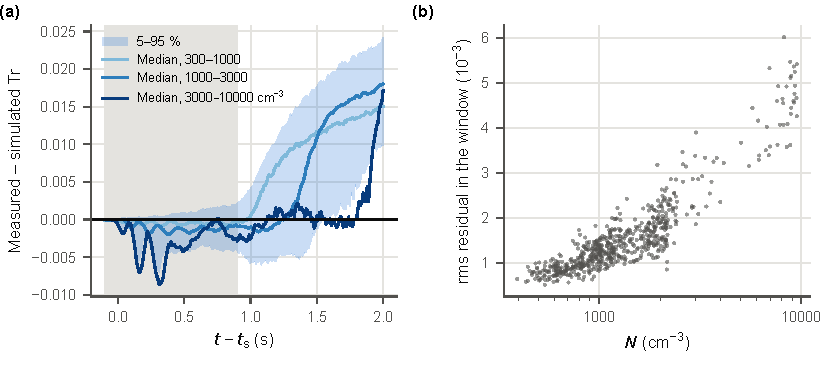
\includegraphics[width=0.85\textwidth]{fig_s_residuals.pdf}
\caption{Residual of the forward model at the posterior median (reference nuisance parameters) for 623
validated cycles. (a) Measured minus simulated Tr against the time after $t_\mathrm{s}$: 5--95\,\% of the
cycles and the median in three ranges of $N$; shaded: inference window. (b) rms residual within the
inference window against $N$.}
\label{fig:s_residuals}
\end{figure}

\begin{table}[!htbp]
\centering
\caption{Fits of $\log_{10}N$ to 104 cycles with different optical paths ($q_w$ fixed at the
hygrometer value, reference nuisance parameters). $N$ relative to that with
$L = 0.18$\,m (median and IQR), median misfit $(\Delta t_\mathrm{s}/20\,\mathrm{ms})^2 +
(\mathrm{rms}\,\Delta\mathrm{Tr}/0.003)^2$, fraction of cycles that fit better than with 0.18\,m, and the
median of the mean residual (measured minus simulated Tr) at $t_\mathrm{s}$ + 1.2--1.5\,s (after the inference
window) for the lowest and the highest third of the cycles in $N$. $L(t)$: path that shrinks as the
warm layer at the wall grows, with $b$ for a tenth of the wall--core temperature difference or with
$b/2$.}
\label{tab:s_path}
\begin{adjustbox}{max width=\textwidth}\small% Generated by Python/paper_si_path.py
\begin{tabular}{llllll}
\toprule
Optical path & $N/N(0.18\,\mathrm{m})$ & Misfit & Better than & \multicolumn{2}{l}{$\Delta$Tr after the window ($10^{-3}$)} \\
\cmidrule(l){5-6}
 & median (IQR) & median & 0.18\,m (\%) & $N < 1100$\,cm$^{-3}$ & $N > 2100$\,cm$^{-3}$ \\
\midrule
0.18\,m (paper) & 1.000 (1.000--1.000) & 0.190 & -- & $+9.2$ & $+3.7$ \\
0.19\,m & 0.932 (0.925--0.939) & 0.232 & 19 & $+9.9$ & $+8.3$ \\
0.17\,m & 1.077 (1.068--1.083) & 0.166 & 59 & $+8.6$ & $-1.2$ \\
0.16\,m & 1.167 (1.151--1.180) & 0.183 & 44 & $+8.2$ & $-4.5$ \\
$L(t)$, $b$ for a tenth & 1.121 (1.109--1.128) & 0.177 & 57 & $+6.7$ & $-6.0$ \\
$L(t)$, $b/2$ & 1.000 (1.000--1.000) & 0.187 & 47 & $+8.8$ & $+3.1$ \\
\bottomrule
\end{tabular}
\end{adjustbox}
\end{table}

Equations~(\ref{M-eq:temperature}) and (\ref{M-eq:growth}) of the paper are integrated with an explicit
time step of 1\,ms. Each of the 12 bins is sub-stepped according to its relaxation rate, and
unactivated haze droplets that relax faster than the time step are kept in equilibrium with the
saturation ratio.
Twelve equal-number bins reproduce Tr of 96 equal-number bins and of 60 log-spaced bins weighted by
the lognormal within $3\times10^{-5}$ in the inference window for the reference values of the aerosol
parameters at
$N$ = 500--8000\,cm$^{-3}$ and $q_w$ = 5.8--9.2\,g\,kg$^{-1}$. The $N$ needed to match differs by
less than 0.01\,\%. Only at the corner of the prior ($r_g$ = 20\,nm, $\sigma_g$ = 2.2,
$\kappa$ = 0.1), where 1--2\,\% of the particles stay unactivated, do the 12 bins activate all
particles, so that $N$ would be up to 2\,\% low (\texttt{Python/\allowbreak paper\_bin\_convergence.py}).

\section{Effective extinction efficiency}
\label{sec:s-qeff}
The photodiode (3.6\,mm $\times$ 3.6\,mm) is replaced by the circle of equal area, of radius
$r_\mathrm{PD} = 3.6\,\mathrm{mm}/\sqrt{\pi} = 2.03$\,mm, centered on the beam. A droplet on the beam at
the distance $\ell$ from the photodiode sees it within the half-angle $\theta_c(\ell) =
\arctan(r_\mathrm{PD}/\ell)$.
For a droplet of radius $a$ in a beam of intensity $I$, the power scattered into this cone is, after
integration over the azimuth \citep[Eqs.~4.74 and 4.77]{bohren1983absorption},
\begin{equation}
P_c = \frac{\pi I}{k^2}\int_0^{\theta_c}\left(|S_1(\theta)|^2 + |S_2(\theta)|^2\right)\sin\theta\,d\theta ,
\end{equation}
with $k = 2\pi/\lambda$, independent of the polarization. Dividing by $\pi a^2 I$ gives the
correction term of Eq.~(\ref{M-eq:qeff}) of the paper.
It is subtracted from $Q_\mathrm{ext}$ and averaged uniformly over $\ell$ = 10--190\,mm, i.e.\ over
the cloud of length $L = 0.18$\,m centered in the flask
with the photodiode 100\,mm from the center.
The correction assumes single scattering (Tr stays above 0.85) and a beam that crosses the flask
through its center.
It neglects the refraction of the scattered light by the curved wall in front of the photodiode and
the angular response of the photodiode.
Both add to the uncertainty of the optical geometry discussed in Sect.~\ref{M-sec:budget} of the paper.

The Mie coefficients and the amplitude functions are computed as in \citet[Eqs.~4.74 and
4.88]{bohren1983absorption} for
$\lambda = 670$\,nm and the refractive index $1.33 + 2\times10^{-8}i$, on a radius grid of 1\,nm up to
30\,\textmu m. The tables of $Q_\mathrm{ext}$ and $Q_\mathrm{eff}$ are averaged over a normal
distribution of the droplet radius of relative standard deviation $s$, weighting by the geometric
cross section.
In Eq.~(\ref{M-eq:kinetic}) of the paper, $D_v' = D_v\,a/(a + a_\mathrm{kin})$ with the kinetic
length $a_\mathrm{kin} = (D_v/\alpha_c)\sqrt{2\pi/(R_v T)}$ (m).
For droplets much larger than $a_\mathrm{kin}$, $a\,da/dt$ hardly depends on $a$ during condensational
growth.
The absolute spread of $a^2$ then stays constant, and $s$ narrows as $a^{-2}$.
For smaller droplets $(a + a_\mathrm{kin})\,da/dt$ is nearly constant instead
($a_\mathrm{kin}$ = 0.2--2\,\textmu m for $\alpha_c$ = 1--0.1), and $s$ narrows more slowly.
In the simulator, $s$ is drawn at $a = 0.69$\,\textmu m, the radius of the first maximum of
$Q_\mathrm{ext}$, and narrows as $a^{-2}$ but not below a prescribed lower bound
(Table~\ref{M-tab:priors} of the paper).
$Q_\mathrm{eff}/Q_\mathrm{ext}$ is 0.97 at $a = 1$\,\textmu m, 0.93 at
2\,\textmu m and 0.89 at 3\,\textmu m (Fig.~\ref{fig:s_qext}).

The narrow droplet spectra assumed here are typical of expansion chambers of this type, in which the
cloud displays coronae with several colored rings that require nearly monodisperse droplets
\citep{aoki2013corona,moteki2013new}. Within the inference window, the spread $s$ has no effect on the
inferred $N$ (Table~\ref{M-tab:uncertainty} of the paper).


\begin{figure}[!htbp]
\centering
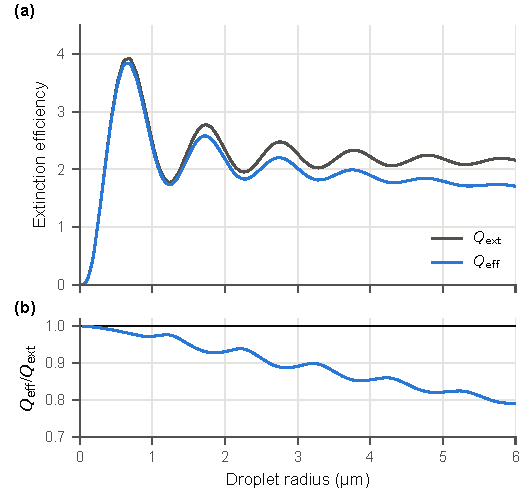
\includegraphics{fig_qext.pdf}
\caption{(a) Extinction efficiency $Q_\mathrm{ext}$ of a water droplet at 670\,nm and the effective
extinction efficiency $Q_\mathrm{eff}$ against droplet radius (relative radius spread $s = 0.04$).
$Q_\mathrm{eff}$ accounts for the light scattered into the cone that the photodiode subtends.
(b) Their ratio.}
\label{fig:s_qext}
\end{figure}

\section{Form of the pressure curve}
\label{sec:s-pform}
This section derives the form of the pressure curve used in Sect.~\ref{M-sec:pressure} of the paper.
Consider a well-mixed chamber of volume $V$ (m$^3$) at pressure $p$ (Pa) pumped at the volumetric speed
\begin{equation}
S_p = S_0\left(1 - \frac{p_\mathrm{off}}{p}\right),
\label{eq:s-pumpspeed}
\end{equation}
which vanishes at the asymptotic pressure $p_\mathrm{off}$ (Pa), the ultimate pressure of the pump
\citep[pp.~87 and 91--92]{eckle1998diaphragm}. $S_p$ (m$^3$\,s$^{-1}$) is the flow of
volume at the pressure and temperature in the chamber, and $S_0$ is the stroke rate times the maximum
volume of the pump chamber. The ultimate pressure of the pump is about half the room pressure
(Sect.~\ref{M-sec:chamber} of the paper), so that $S_p$ is only about half of $S_0$ even at the start
of the expansion. The $p_\mathrm{off}$ fitted with Eq.~(\ref{M-eq:pressure}) of the paper is not well
determined and need not equal this value (Sect.~\ref{sec:s-pressure}).
This form describes a piston or diaphragm pump in which the gas left in the dead volume at the end of
each stroke re-expands and reduces the intake.
It assumes that the re-expansion is isothermal and that the gas enters the pump at the temperature
of the chamber. The intake then vanishes at $p_\mathrm{off} = p_0 V_\mathrm{D}/V_\mathrm{P}$, where
$p_0$ (Pa) is the outlet pressure and $V_\mathrm{D}/V_\mathrm{P}$ is the ratio of the dead volume to
the maximum volume of the pump chamber.
The pump removes the gas of density $\rho$ (kg\,m$^{-3}$) from the volume, and the gas left in the
volume expands adiabatically:
\begin{equation}
\frac{\mathrm{d}\rho}{\mathrm{d}t} = -C(t)\,\frac{S_p}{V}\,\rho, \qquad
\frac{\mathrm{d}p}{p} = \gamma\,\frac{\mathrm{d}\rho}{\rho}.
\label{eq:s-massbalance}
\end{equation}
Here $C(t)$ is the effective pumping speed at the chamber normalized by its value
with the valve fully open. It includes the pressure drop across the valve and the tubing.
$\gamma$ is the ratio of the specific heats. The second relation is the dry adiabat
\citep[Eq.~20]{moteki2013new} combined with the ideal-gas law.
Equations~(\ref{eq:s-pumpspeed}) and (\ref{eq:s-massbalance}) together give
\begin{equation}
\frac{\mathrm{d}p}{\mathrm{d}t} = -C(t)\,\frac{p - p_\mathrm{off}}{\tau}, \qquad
\tau = \frac{V}{\gamma S_0}\ (\mathrm{s}).
\end{equation}
Integration from $p(t_0) = p_\mathrm{ini}$ gives
\begin{equation}
p(t) = p_\mathrm{off} + (p_\mathrm{ini} - p_\mathrm{off})
\exp\!\left(-\frac{1}{\tau}\int_{t_0}^{t} C(t')\,\mathrm{d}t'\right),
\label{eq:s-singleexp}
\end{equation}
where the valve-opening onset $t_0$ (s) is the time at which the valve starts to open.
With an instantaneous opening ($C = 1$ for $t \ge t_0$) this is the single exponential first fitted to the
recorded pressure (Sect.~\ref{M-sec:pressure} of the paper).

The recorded decay deviates from Eq.~(\ref{eq:s-singleexp}) also after the valve has opened. Possible
reasons are the pressure dependence of $C$, heat from the walls of the flask in the later
part of the record and a re-expansion in the pump that is not isothermal. The adiabatic expansion
assumed above holds best during the first seconds, when the cloud forms. Equation~(\ref{M-eq:pressure}) of
the paper represents the deviation empirically by a second exponential with the same $C(t)$.

Four forms of the pressure curve were fitted to the recorded pressure of all 3132 cycles, each with
$p_\mathrm{ini}$ fixed and the valve-opening onset $t_0$ free:
a single exponential with instantaneous opening ($f_1 = 1$, $\Delta t_\mathrm{open} = 0$), the same with the
linear ramp of $C$ ($f_1 = 1$), two exponentials with instantaneous opening
($\Delta t_\mathrm{open} = 0$), and Eq.~(\ref{M-eq:pressure}) of the paper.
For the forms with instantaneous opening, $t_0$ was allowed up to 1\,s after the upper bound of
Sect.~\ref{M-sec:pressure} of the paper so that the bound does not handicap them.
Their rms residuals over the first 2\,s are compared in Sect.~\ref{M-sec:pressure} and
Fig.~\ref{M-fig:pressure} of the paper.
Over the whole record the medians are
3.0, 2.8, 1.7 and 0.65\,hPa (\texttt{Python/\allowbreak paper\_pressure\_models.py}). Neither the valve
opening nor the second exponential suffices alone.

The recorded pressure is concave down during the first 0.5--0.7\,s and concave up afterward
(Fig.~\ref{M-fig:pressure}a of the paper). Shortly after $t_0$, the integral of $C$ is small and
Eq.~(\ref{M-eq:pressure}) of the paper gives
\begin{equation}
p(t) \approx p_\mathrm{ini} - (p_\mathrm{ini} - p_\mathrm{off})
\left[\frac{f_1}{\tau_1} + \frac{1 - f_1}{\tau_2}\right]\frac{(t - t_0)^2}{2\Delta t_\mathrm{open}},
\end{equation}
a quadratic, concave-down start of the drop that comes from the linear growth of $C$
while the valve
opens. A sum of decaying exponentials that starts at $t_0$ is concave up throughout and falls most
steeply at $t_0$, so that it cannot reproduce this start. The fit with instantaneous opening instead
moves $t_0$ later and cuts across the curve (inset of Fig.~\ref{M-fig:pressure}a of the paper). The
response of the sensor and of the tubing to it would also round the start of the drop. The stated
time constant of the sensor is 10\,ms (to 90\,\% of a pressure step). The Poiseuille time constant of
the tubing
(Sect.~\ref{M-sec:sensors} of the paper) with the sensor volume and the acoustic delay are each about
2\,ms. All three are much shorter than the 0.5--0.7\,s observed.
After full opening, the integral of $C$ is the triangle $\Delta t_\mathrm{open}/2$ plus the time since
full opening, so that the pressure then decays as if the valve had opened instantly at
$t_0 + \Delta t_\mathrm{open}/2$.

\begin{table}[!htbp]
\centering
\caption{Bias of the estimates if the pressure were described by a single exponential with
instantaneous opening, for synthetic $q_w$ with the pressure curves and initial states
($T_\mathrm{ini} = 296$\,K) of the two cycles of Fig.~\ref{M-fig:cycle} of the paper and
$N = 1000$ and 5000\,cm$^{-3}$ (ranges over the four combinations). $t_\mathrm{s}$: onset of the extinction.
The measurements covered $q_w$ = 5.8--9.2\,g\,kg$^{-1}$.}
\label{tab:s_pform}
\small
\begin{tabular}{rccc}
\toprule
$q_w$ (g\,kg$^{-1}$) & $t_\mathrm{s}$ (s) & $q_{w,\mathrm{single}}/q_w$ & $N_\mathrm{single}/N$ \\
\midrule
6  & 1.58--1.67 & 1.013--1.017 & 0.996--0.997 \\
8  & 1.23--1.30 & 1.009--1.010 & 0.999--1.002 \\
10 & 0.98--1.03 & 1.001--1.003 & 1.001 \\
12 & 0.78--0.83 & 0.992--0.997 & 1.001--1.009 \\
14 & 0.61--0.66 & 0.982--0.990 & 1.002--1.014 \\
16 & 0.46--0.51 & 0.979--0.985 & 1.004--1.016 \\
\bottomrule
\end{tabular}
\end{table}

The effect of the form on the estimates was tested with the forward model, using the script
\texttt{Python/\allowbreak paper\_pressure\_form\_effect.py}.
For a recorded cycle, Tr was simulated with the fit
of Eq.~(\ref{M-eq:pressure}) of the paper and the estimated $q_w$ and $N$ (reference nuisance
parameters) and taken as the truth. The pressure curve was then replaced by the fit of the single
exponential with instantaneous opening to the same record, and $q_w$ and $N$ were refitted by
minimizing the rms difference of Tr over the inference window. For 30 cycles spread evenly in time over the
measurement period, the single exponential gives $q_w$ higher by 1.6\,\% (median; range 0.5--2.2\,\%) and
$N$ within
0.5\,\% of the truth.
The error of the pressure shifts the time of saturation, and $q_w$ absorbs most of this shift.
The refitted curves match the truth to within 0.0007 in Tr. This is below the rms residual of the
forward model within the inference window (median $1.4\times10^{-3}$; Sect.~\ref{sec:s-thermo}), so the
bias would not show in the fit.
In humid air, the cloud forms earlier and the inference window
overlaps the opening of the valve. With the pressure curves and initial states of the two cycles of
Fig.~\ref{M-fig:cycle} of the paper and synthetic $q_w$ beyond the evaluated range
(Table~\ref{tab:s_pform}), the bias in $q_w$ changes sign as the window moves across the residual of
the single exponential, and that in $N$ reaches up to $+1.6$\,\% when the cloud forms within 0.7\,s.
Equation~(\ref{M-eq:pressure}) of the paper is therefore needed most in humid air.


\section{Pressure-curve library and parameter degeneracy}
\label{sec:s-pressure}
Equation~(\ref{M-eq:pressure}) of the paper was fitted to the recorded pressure of every cycle. The fits
reproduce the recorded curves (Sect.~\ref{M-sec:pressure} of the paper), but their parameters are
not unique (Fig.~\ref{fig:s_pressure}a).
Over the 3132 cycles the asymptotic pressure $p_\mathrm{off}$ ranges over 0--421\,hPa and the second
time constant $\tau_2$ over 3.3--87.5\,s.
They trade off against each other and against $f_1$ because the curves are recorded only for 10\,s.
The curves themselves
are much more uniform (Fig.~\ref{fig:s_pressure}b, c): 90\,\% of the relative pressure drops lie within
$-1.7$ to $+1.6$\,\% of the median at 1\,s and within $-0.6$ to $+0.8$\,\% at 4\,s. The observation vector
therefore contains the pressure drop of the fitted curve at 11 fixed times rather than the fit
parameters, and the simulator draws whole fitted curves (with their parameters) from a library of
the recorded cycles of the days used to train the estimator (Sect.~\ref{M-sec:lodo} of the paper),
scaled in drop and time by up to $\pm5$\,\% and with the
valve-opening duration $\Delta t_\mathrm{open}$ shifted by up to $\pm0.05$\,s
(Table~\ref{M-tab:priors} of the paper).
Changes of
the pump or valve within this range are thus absorbed by the inference without retraining.


\begin{figure}[!htbp]
\centering
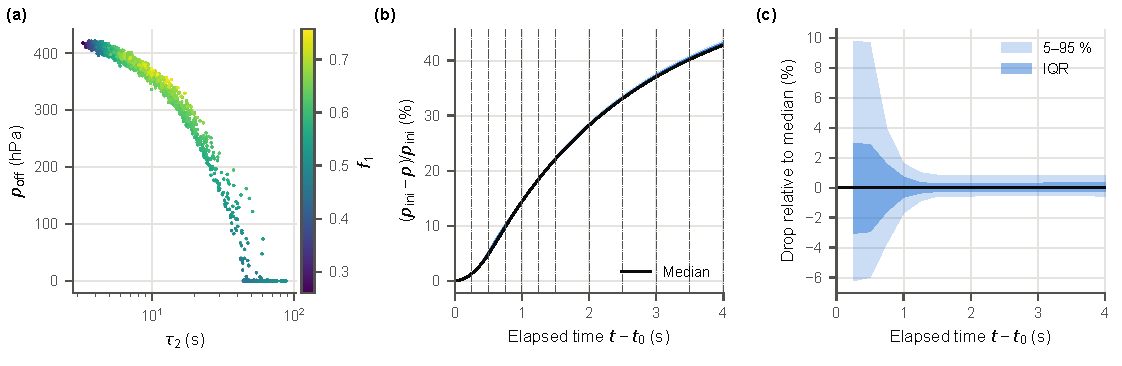
\includegraphics[width=\textwidth]{fig_s_pressure.pdf}
\caption{Fits of the pressure model to all recorded cycles (31 Oct 12:18 -- 2 Nov 16:49).
(a) Asymptotic pressure $p_\mathrm{off}$ against the second time constant $\tau_2$, colored by the
fraction $f_1$ of the first exponential: the parameters trade off against each other. (b) The fitted
curves as the relative pressure drop (300 random cycles) and their median. Dotted lines mark the 11
times used in the observation vector. (c) Spread of the drop at those times relative to the median.}
\label{fig:s_pressure}
\end{figure}

\section{Training of the neural posterior estimator}
\label{sec:s-npe}
Each estimator uses 30\,000 draws from the priors (Table~\ref{M-tab:priors} of the paper). In
24\,304--24\,317 of them (81\,\%) the simulated cloud reaches Tr = 0.985 within the simulated 4.2\,s, so
that the
onset $t_\mathrm{s}$ and the observation vector $\bm{y}$ are defined.
The others are discarded.
This restricts the posterior to cycles that produce a measurable cloud, as all recorded cycles did.
The last 2000 usable pairs are held out
(Fig.~\ref{fig:s_heldout}), and the remaining 22\,304--22\,317 are used for training.

\begin{figure}[!htbp]
\centering
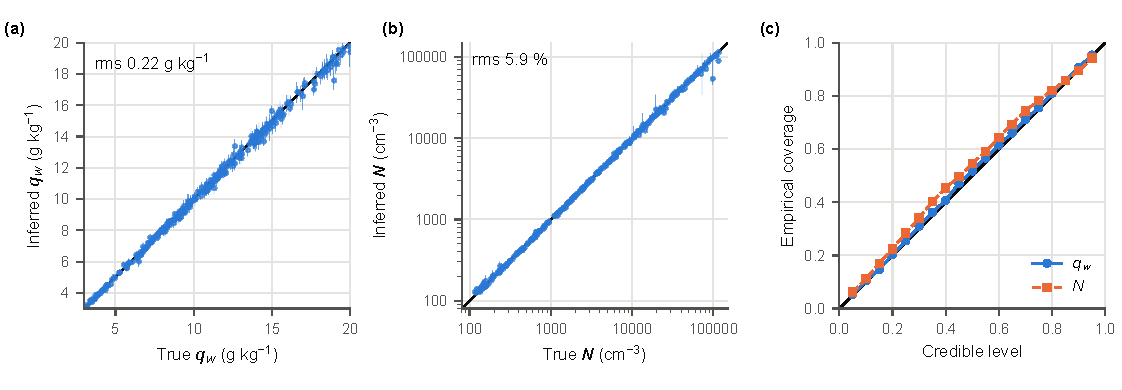
\includegraphics[width=\textwidth]{fig_heldout.pdf}
\caption{Posterior on 2000 simulations not used in training (estimator trained on 31 Oct--1 Nov).
(a) $q_w$ and (b) $N$: posterior median and 90\,\% credible interval against the true value (300
random cases shown). (c) Empirical coverage of central credible intervals.}
\label{fig:s_heldout}
\end{figure}

The posterior $q_\phi(\bm{\psi}\mid \bm{y})$ is a neural spline flow \citep{durkan2019neural} built with
\texttt{sbi} 0.27.0 and PyTorch 2.14 \citep{tejerocantero2020sbi,boelts2025sbi}, with the default settings of
its neural spline flow. The flow maps a standard normal distribution onto the posterior through a chain
of invertible monotonic functions, whose parameters a neural network computes from $\bm{y}$. It has five
rational-quadratic spline transforms with ten bins. Each transform is conditioned on $\bm{y}$ through a
residual network with 50 hidden units in two blocks. $\bm{\psi}$ and the 115 components of $\bm{y}$ are
z-scored independently with the means and standard deviations of the training set. The flow is trained with
Adam
(learning rate \num{5e-4}, batches of 200, gradient norm clipped at 5) on 90\,\% of the training
pairs and stopped when the loss on the other 10\,\% has not improved for 20 epochs (passes through
the training set). The prior of
$\bm{\psi}$ is a uniform distribution (Table~\ref{M-tab:priors} of the paper), and samples outside it are
rejected.
On a separate laptop (Intel Core i7-13700H CPU), the 30\,000 simulations take 2--3\,min with 11 parallel
processes, and the training converges after 80--130 epochs in 4--8\,min.

A recorded cycle is evaluated by drawing 1000 samples from $q_\phi(\bm{\psi}\mid \bm{y})$, from which the
median and the 5--95\,\% interval of $q_w$ and $\log_{10}N$ are taken. The complete processing of a
cycle (onset detection, fit of the pressure curve, observation vector and sampling) takes 0.08\,s
(median; 95th percentile 0.16\,s) on the laptop used for the measurements.

The onset time $t_\mathrm{s}$ of the observation vector is defined on the transmittance $\mathrm{Tr} = I/I_0$
(Sect.~\ref{M-sec:obs} of the paper). The baseline is the median of Tr from the start of the expansion
phase to $t_0$. $t_\mathrm{s}$ is the last time before Tr first falls to 0.985 at which Tr is still above the
baseline minus a noise margin of five standard deviations of the baseline (at least $10^{-3}$),
interpolated linearly between samples. The simulated curves are reduced by the
same code.

On the 2000 held-out simulations (Fig.~\ref{fig:s_heldout}), the rms error of the posterior median is
0.22\,g\,kg$^{-1}$ for $q_w$ and 5.9\,\% for $N$.
The central credible intervals contain the true value at their nominal rate (90\,\% intervals:
91\,\% for $q_w$ and 90\,\% for $N$).
This coverage test is recommended for checking whether the credible intervals of simulation-based
inference contain the true value at their stated probability \citep{talts2018validating,hermans2022trust}.


\section{Validation of the individual estimators}
\label{sec:s-models}
Four estimators were trained, identical except for the recorded pressure curves of their simulator
library: one for each held-out day (trained on the other two days, e.g.\ on 31 Oct--1 Nov
for 2 Nov) and one trained on all days. Table~\ref{tab:s_models} compares them
on the cycles of Fig.~\ref{M-fig:validation}
of the paper. On a given day, the estimator that has not seen that day and the estimators
that have seen it give nearly the same result: for $N/N_\mathrm{CPC}$ the medians differ by at most
0.02, and for $q_w/q_{w,\mathrm{hyg}}$ by at most 0.011. The estimates therefore depend little on whether the
day was used in training, and the leave-one-day-out result of the paper is not limited by the
number of recorded pressure curves. Per cycle, the leave-one-day-out estimate of $N$ is higher than that
of the estimator trained on all days by 0.8\,\% (median; IQR $-0.2$ to $+1.7$\,\%).
Retraining the 2 Nov estimator on the same simulations with three other random seeds
(\texttt{Python/\allowbreak paper\_seed\_variability.py}) changes the median $N/N_\mathrm{CPC}$ on 2 Nov
from 0.981 to 0.972--0.979 and $q_w/q_{w,\mathrm{hyg}}$ from 0.999 to 1.003--1.004. Per cycle, $N$
is lower by 0--0.8\,\% (median). The differences between estimators trained on different days are
thus of the same size as those between retrainings. The daily
medians of $N/N_\mathrm{CPC}$ (0.98--1.04) differ by more than the estimators do. These differences are
discussed in Sect.~\ref{M-sec:limitations} of the
paper.

\begin{table}[!htbp]
\centering
\caption{Validation of the individual estimators on each day (same cycles as Fig.~\ref{M-fig:validation}
of the paper). $r$: Pearson's correlation coefficient of $N$ with $N_\mathrm{CPC}$. In 90\,\% CI: percentage
of cycles with $N_\mathrm{CPC}$
inside the 90\,\% credible interval of $N$.}
\label{tab:s_models}
\begin{adjustbox}{max width=\textwidth}\small% Generated by Python/paper_si_table_models.py
\begin{tabular}{llrllrl}
\toprule
Estimator & Day & Cycles & $N/N_\mathrm{CPC}$ & $r$ & In 90\,\% CI & $q_w/q_{w,\mathrm{hyg}}$ \\
 & & & median (IQR) & & (\%) & median (IQR) \\
\midrule
Leave-one-day-out & 31 Oct & 700 & 1.041 (0.995--1.099) & 0.993 & 47 & 0.989 (0.979--0.999) \\
 & 1 Nov & 1440 & 0.988 (0.943--1.043) & 0.988 & 41 & 1.000 (0.989--1.010) \\
 & 2 Nov & 974 & 0.981 (0.940--1.015) & 0.998 & 54 & 0.999 (0.989--1.008) \\
 & All & 3114 & 0.995 (0.950--1.046) & 0.997 & 46 & 0.997 (0.987--1.007) \\
\midrule
Trained on 31 Oct--1 Nov & 31 Oct$^{a}$ & 700 & 1.046 (0.998--1.105) & 0.993 & 46 & 0.984 (0.974--0.994) \\
 & 1 Nov$^{a}$ & 1440 & 1.003 (0.962--1.052) & 0.989 & 54 & 0.996 (0.986--1.004) \\
 & 2 Nov & 974 & 0.981 (0.940--1.015) & 0.998 & 54 & 0.999 (0.989--1.008) \\
 & All & 3114 & 1.002 (0.960--1.052) & 0.998 & 52 & 0.994 (0.984--1.004) \\
\midrule
Trained on all days & 31 Oct$^{a}$ & 700 & 1.028 (0.981--1.084) & 0.992 & 49 & 0.992 (0.981--1.003) \\
 & 1 Nov$^{a}$ & 1440 & 0.987 (0.945--1.038) & 0.988 & 48 & 1.004 (0.992--1.015) \\
 & 2 Nov$^{a}$ & 974 & 0.967 (0.929--1.001) & 0.998 & 48 & 1.010 (1.001--1.019) \\
 & All & 3114 & 0.987 (0.944--1.037) & 0.998 & 48 & 1.004 (0.992--1.015) \\
\bottomrule
\multicolumn{7}{l}{\footnotesize $^{a}$ Day used in training.}\\
\end{tabular}
\end{adjustbox}
\end{table}

\section{Variations of the ratio to the CPC}
\label{sec:s-hvac}
The ratio $N/N_\mathrm{CPC}$ has a median of 0.995, and its median over consecutive 3-h intervals ranges
from 0.95 to 1.09. Binned
by the hygrometer mixing ratio (Fig.~\ref{fig:s_humidity}a), its median is 1.08 at 5.5--6.0\,g\,kg$^{-1}$,
0.95 at 7.5--8.0\,g\,kg$^{-1}$ and 1.00--1.03 above 8.5\,g\,kg$^{-1}$. This pattern does not isolate an
effect of humidity. The dry bins (below 7\,g\,kg$^{-1}$) come from 31 Oct and 1 Nov, when the driest air
also had the lowest particle number concentration (nights): within each of these days the logarithm of
the ratio is
correlated with the mixing ratio ($r = -0.45$ and $-0.50$) and with the logarithm of $N_\mathrm{CPC}$
($r = -0.50$ and $-0.41$). The humid bins (above 8.5\,g\,kg$^{-1}$) come from 2 Nov and coincide with the
periods without air conditioning described below. Humidity, particle number concentration, time of day
and the state
of the air conditioning thus varied together. With at least 20 cycles per bin, the differences
between the bins are larger than their statistical uncertainty, but they are confounded with these
variables. Binned by $N_\mathrm{CPC}$ (Fig.~\ref{fig:s_humidity}b), the median is 1.05--1.06 below
750\,cm$^{-3}$, 0.96--0.98 at 1300--4200\,cm$^{-3}$ and 0.99--1.01 above 5600\,cm$^{-3}$ (window open on
2 Nov).

\begin{figure}[!htbp]
\centering
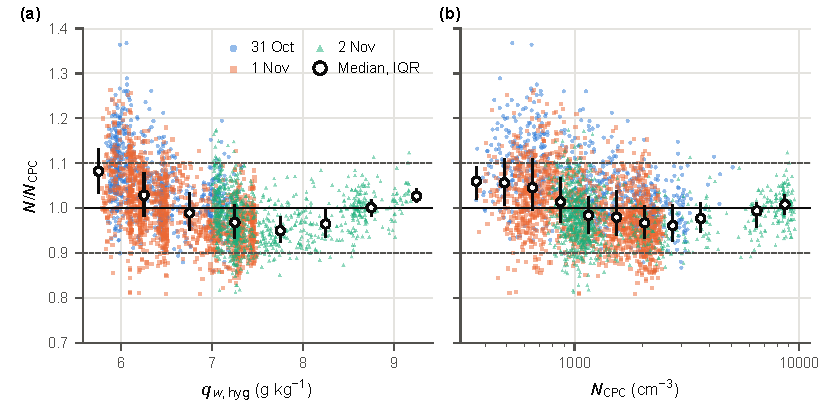
\includegraphics[width=\textwidth]{fig_humidity.pdf}
\caption{$N/N_\mathrm{CPC}$ against (a) the hygrometer mixing ratio and (b) $N_\mathrm{CPC}$ for the
cycles of Fig.~\ref{M-fig:validation} of the paper, with the median and IQR in bins of
0.5\,g\,kg$^{-1}$ and of 1/8 decade (at least 20 cycles).}
\label{fig:s_humidity}
\end{figure}

On 2 Nov the room air was changed deliberately (Fig.~\ref{fig:s_hvac}).
The room (about 90\,m$^3$) has a portable air purifier without ion generation. It also has two air
conditioners and a dehumidifier, which were always switched together (``air conditioning'' below).
The window was opened and closed.
The
inlets of the chamber, the CPC and the hygrometer were 5--10\,cm apart at the same height, out of the
direct flow of the air conditioners. Figure~\ref{fig:s_hvac} starts at 09:30, after the laser had been
realigned at 09:27.

\begin{figure}[!htbp]
\centering
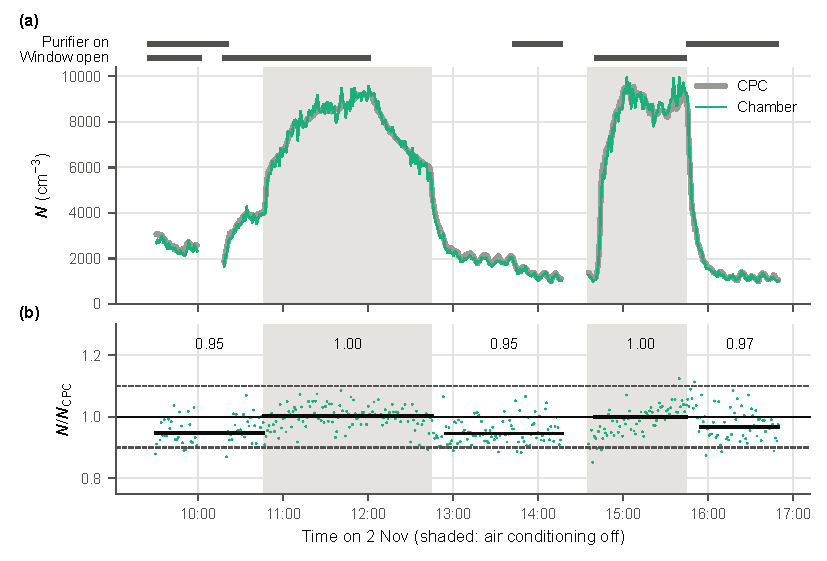
\includegraphics[width=0.85\textwidth]{fig_s_hvac.pdf}
\caption{Room-air experiments on 2 Nov (estimator trained on 31 Oct--1 Nov).
(a) $N$ and $N_\mathrm{CPC}$.
Bars mark the open window and the air purifier.
(b) $N/N_\mathrm{CPC}$ per cycle with the median of each period.
Shaded: air conditioning off.}
\label{fig:s_hvac}
\end{figure}

Opening the window raised $N_\mathrm{CPC}$ from about 1000 to 9000\,cm$^{-3}$, and the air
conditioning and the air purifier lowered it.
The chamber followed all changes.
However, the ratio $N/N_\mathrm{CPC}$ changed with the air conditioning.
Its median was 1.002 and 0.999 in the two periods with the air
conditioning off and 0.947, 0.945 and 0.966 in the three periods with it on, and it changed within
5--10\,min of switching.
The periods without air conditioning largely coincide with the open window. With the air
conditioning off, the median was 1.00 both with the window open (10:46--12:01) and closed
(12:02--12:44). With the air conditioning on, switching the air purifier changed the median by at
most about 0.03, without a consistent sign.
However, with the air conditioning off the air was also more humid (period medians
8.6--9.0 against 7.6--8.1\,g\,kg$^{-1}$) and had a higher particle number concentration.
This effect therefore cannot be separated from the
variation with humidity in Fig.~\ref{fig:s_humidity}a.
The cause was not identified.
Possible explanations are particles
emitted or modified by the air conditioners that the CPC counts but that activate less readily in the
chamber, and size distributions outside the priors of the simulator.
From 10:00 to 10:18 water was nebulized near the inlets in a separate test.
It produced short dense plumes that reached the inlets of the chamber and of the CPC at different times.
The air sealed in the chamber during the flushing and the air of the 20-s median of the CPC therefore
differed.
These 18 cycles are excluded, as in the paper.



\section{Sensitivity to nuisance parameters}
\label{sec:s-nuisance}
The effect of each nuisance parameter on $N$ was evaluated directly with the forward model, outside
the neural posterior estimator. For 104 cycles spread evenly over the range of $q_{w,\mathrm{hyg}}$
(31 Oct--2 Nov), $\log_{10}N$ was fitted with $q_w$ fixed at $q_{w,\mathrm{hyg}}$ and the recorded
pressure curve.
The misfit $(\Delta t_\mathrm{s}/20\,\mathrm{ms})^2 + (\mathrm{rms}\,\Delta\mathrm{Tr}/0.003)^2$ was minimized
over $\log_{10}N$ and over a time shift of the simulated curve within $\pm0.02$\,s.
Here $\Delta t_\mathrm{s}$ is the difference in the onset of the extinction, and
$\mathrm{rms}\,\Delta\mathrm{Tr}$
is the rms difference of Tr over the inference window.
The limit of $\pm0.02$\,s is twice the standard deviation of the error of $t_0$ in the simulator
(Table~\ref{M-tab:priors} of the paper).
The fit was made with the reference nuisance parameters
($r_g = 40$\,nm, $\sigma_g = 1.8$, $\kappa = 0.3$, $\alpha_c = 0.3$, droplet-radius spread 0.04 with a
lower bound of 0.01) and again with one parameter at a time at either edge of its prior.
Table~\ref{tab:s_nuisance}
gives the median and interquartile range over the cycles of $N(\text{edge})/N(\text{reference})$, and the
median misfit.

\begin{table}[!htbp]
\centering
\caption{Sensitivity of $N$ to the nuisance parameters (104 cycles): ratio of the best-fit $N$ with one
parameter at an edge of its prior to that with the reference set, and median misfit.}
\label{tab:s_nuisance}
\small% Generated by Python/paper_si_nuisance.py
\begin{tabular}{llll}
\toprule
Parameter & Edge & $N/N_\mathrm{ref}$, median (IQR) & Misfit, median \\
\midrule
Reference set & -- & 1 & 0.19 \\
Condensation coefficient $\alpha_c$ & 0.1 & 1.118 (1.058--1.154) & 1.01 \\
 & 1 & 0.972 (0.957--0.987) & 0.20 \\
Geometric mean dry radius $r_g$ & 20\,nm & 0.987 (0.984--1.002) & 0.24 \\
 & 80\,nm & 1.021 (0.994--1.037) & 0.27 \\
Geometric standard deviation $\sigma_g$ & 1.4 & 1.000 (0.996--1.002) & 0.20 \\
 & 2.2 & 1.000 (0.999--1.006) & 0.18 \\
Hygroscopicity $\kappa$ & 0.1 & 0.993 (0.991--0.999) & 0.21 \\
 & 0.7 & 1.008 (1.000--1.011) & 0.19 \\
Droplet-radius spread & 0.015 & 1.000 (0.999--1.000) & 0.19 \\
 & 0.10 & 1.000 (1.000--1.001) & 0.19 \\
Lower bound of the spread & 0.003 & 1.000 (1.000--1.000) & 0.19 \\
 & 0.03 & 1.000 (0.998--1.003) & 0.18 \\
\bottomrule
\end{tabular}

\end{table}

The condensation coefficient has the largest effect: at $\alpha_c = 0.1$ the droplets grow more
slowly, and the fit needs 12\,\% more of them to reproduce the curve.
These fits are worse than the reference ones and better in only 4\,\% of the cycles.
The curves thus disfavor $\alpha_c = 0.1$ but do not distinguish 0.3 from 1 (misfit 0.19 and 0.20). The
condensation coefficient
trades off against the time shift: with the shift held at zero, $N$ at $\alpha_c = 0.1$ would be 16\,\%
higher. The aerosol parameters change $N$ by at most 2.1\,\%, and the spread of the droplet radius and
its lower bound have no effect within the
inference window. In the neural posterior estimator all these parameters are marginalized over their
priors, weighted by how well they reproduce the curve. The effects in Table~\ref{tab:s_nuisance}
indicate the size of their contribution to the estimates.

The same fits were repeated with $q_w$ fixed at 0.97 and 1.03 times $q_{w,\mathrm{hyg}}$
(\texttt{Python/\allowbreak paper\_\allowbreak qw\_\allowbreak sensitivity.py}).
The sensitivity $\mathrm{d}\ln N/\mathrm{d}\ln q_w$ is $-2.3$ (median; IQR $-3.9$ to $-1.3$).
An error of 3\,\% in $q_w$ thus changes $N$ by about 5--7\,\% in the opposite direction: a higher
$q_w$ makes the droplets grow faster, so fewer of them reproduce the curve.
The fits with $q_{w,\mathrm{hyg}}$ itself are the best (median misfit 0.19 against 1.21 and 0.48
for the factors 0.97 and 1.03).


\clearpage
\section{Activation cutoff size}
\label{sec:s-cutoff}
For every tenth cycle of the $N$ validation (312 cycles), the forward model was run with the inferred
$q_w$ and $N$, the recorded pressure curve and the reference nuisance parameters. The peak
saturation ratio $S_\mathrm{max}$ and the temperature at the peak give the smallest dry diameter
whose critical saturation ratio by $\kappa$-Köhler theory \citep{petters2007single} does not exceed
$S_\mathrm{max}$.
For $\kappa = 0$ (insoluble but wettable particles) the Kelvin equation is used.
$S_\mathrm{max} - 1$ ranges over 21--75\,\% (5--95\,\% of the cycles; median 51\,\%) and decreases
with $N$ because more droplets deplete the vapor sooner (Fig.~\ref{fig:s_cutoff}a).
The peak is reached
at $-11$ to $+6$\,$^\circ$C. The corresponding cutoff diameters (5--95\,\%, median) are 4.5--12.1\,nm
(6.0\,nm) for $\kappa = 0$, 3.1--6.7\,nm (3.9\,nm) for $\kappa = 0.1$, 2.5--5.2\,nm (3.1\,nm) for
$\kappa = 0.3$ and 2.2--4.3\,nm (2.6\,nm) for $\kappa = 0.6$.
For soluble particles they are at or below the nominal 7\,nm of the TSI 3022A (Fig.~\ref{fig:s_cutoff}b).

\begin{figure}[!htbp]
\centering
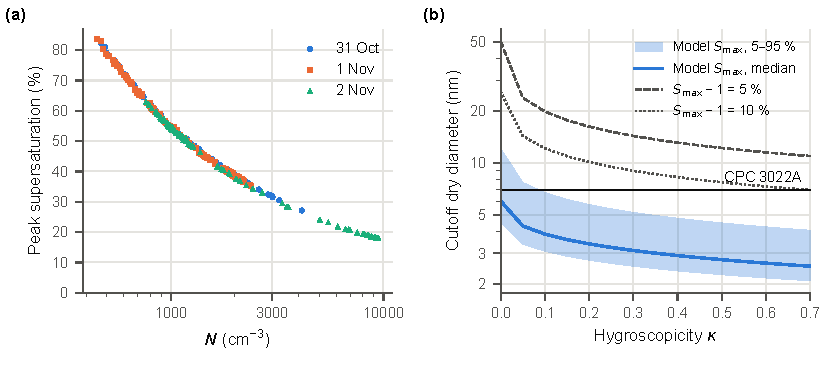
\includegraphics[width=0.85\textwidth]{fig_s_cutoff.pdf}
\caption{Counting cutoff from theory for every tenth validated cycle (312 cycles). (a) Peak
supersaturation of the forward model (inferred $q_w$ and $N$, recorded pressure curve, reference
nuisance parameters) against $N$. (b) Smallest dry diameter whose critical supersaturation is reached
($\kappa$-K\"ohler; $\kappa = 0$: insoluble, wettable particle) as median and 5--95\,\% of the
cycles and for lower peak supersaturations as a sensitivity.
The horizontal line is the nominal 7-nm 50\,\% cutoff of the
TSI 3022A.}
\label{fig:s_cutoff}
\end{figure}

These values are uncertain. Köhler theory is extrapolated below 10\,nm (surface tension, slightly
soluble organics). The peak is reached 0.3\,s (highest $N$) to 1.4\,s (lowest $N$) after
saturation. In 19\,\% of the cycles, mainly at the lowest $N$, it
comes after the end of the inference window, where the measured Tr departs from the model
(Sect.~\ref{M-sec:obs} of the paper).
Figure~\ref{fig:s_cutoff}b therefore also shows the cutoff for lower peaks.
At $S_\mathrm{max} - 1 = 5$\,\% it would be about 14\,nm for
$\kappa = 0.3$.
The saturation ratios reached are up to about 1.75 (95th percentile of the cycles; up to 1.84 at
the lowest $N$).
In particle-free air, drops form only above a saturation ratio of about 4
\citep{wilson1897condensation}, so ions and other nuclei that are not particles are not counted.




Figure~\ref{fig:s_envelope} extends these calculations beyond the evaluated range, using the script
\texttt{Python/\allowbreak paper\_si\_envelope.py}. The pressure curve of the
high-$N$ cycle of Fig.~\ref{M-fig:cycle} of the paper was used with $T_\mathrm{ini}$ = 10, 23 and
30\,$^\circ$C, $q_w$ from 2\,g\,kg$^{-1}$ to saturation and $N$ = 50--30\,000\,cm$^{-3}$ (reference nuisance
parameters). The peak supersaturation falls with $N$ and rises as $T_\mathrm{ini}$ falls. For
$\kappa = 0.1$ the cutoff stays below about 9\,nm up to 10$^4$\,cm$^{-3}$ and reaches 9--13\,nm at
3$\times10^4$\,cm$^{-3}$. A measurable cloud (Tr reaching 0.985) needs more particles in drier air: at
23\,$^\circ$C about 90, 160, 320 and 560\,cm$^{-3}$ at $q_w$ = 9, 6, 4 and 3\,g\,kg$^{-1}$, and about
2200\,cm$^{-3}$ at 2\,g\,kg$^{-1}$. At 30\,$^\circ$C no cloud forms at 2\,g\,kg$^{-1}$. At 10\,$^\circ$C
in humid air ($q_w > 5$\,g\,kg$^{-1}$) with fewer than about 100\,cm$^{-3}$, the peak saturation ratio
exceeds 4, so that drops
could form also without particles. The estimator covers only its priors ($q_w$ = 3--20\,g\,kg$^{-1}$,
$T_\mathrm{ini}$ = 288--303\,K) and would have to be retrained for other conditions.

\begin{figure}[!htbp]
\centering
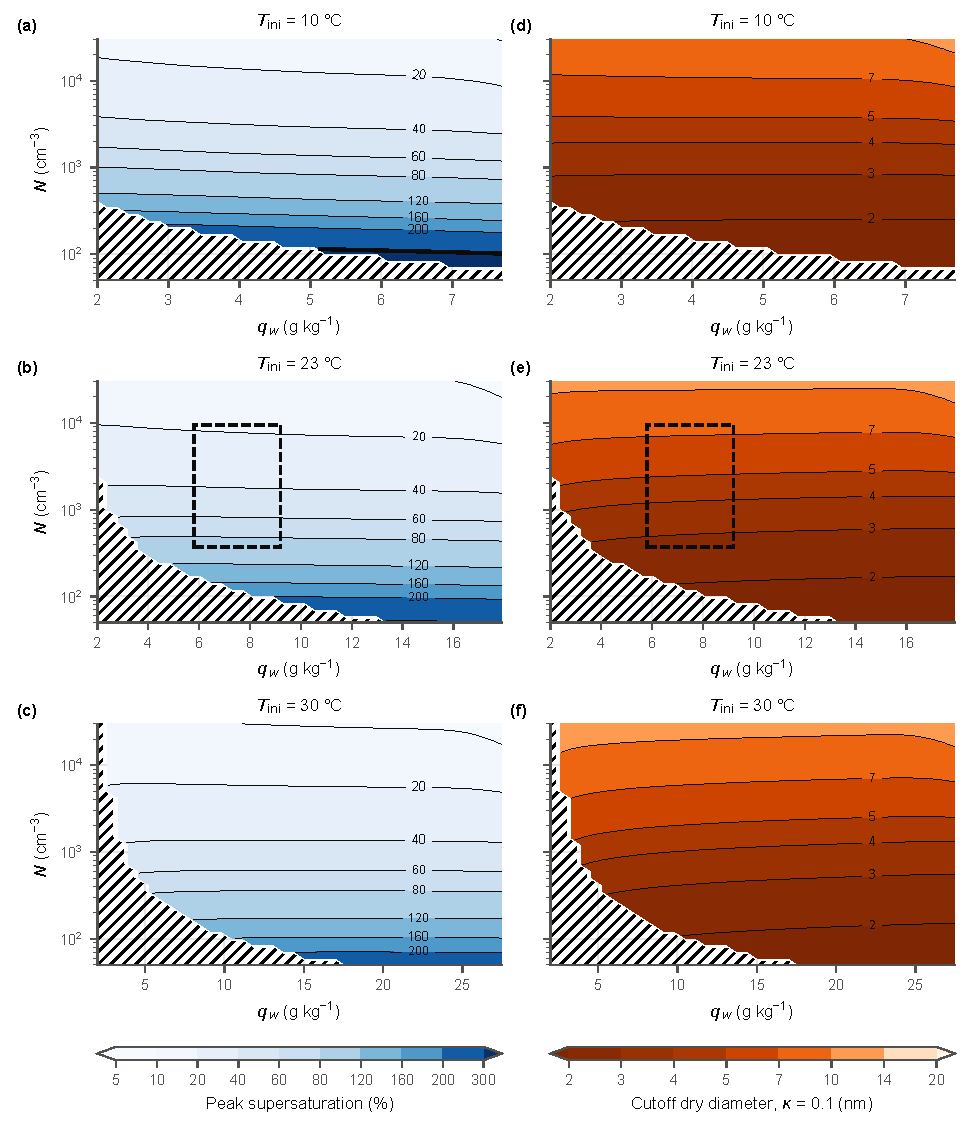
\includegraphics[width=\textwidth]{fig_s_envelope.pdf}
\caption{Operating range from the forward model for the pressure curve of the high-$N$ cycle of
Fig.~\ref{M-fig:cycle} of the paper and reference nuisance parameters. (a--c) Peak supersaturation and
(d--f) smallest activated dry diameter for $\kappa = 0.1$ against $q_w$ and $N$, for
$T_\mathrm{ini}$ = 10, 23 and 30\,$^\circ$C (top to bottom). Hatched: no measurable cloud (Tr does not reach
0.985).
Thick line in (a): saturation ratio 4. Dashed box in (b, e): range of the measurements.}
\label{fig:s_envelope}
\end{figure}

\clearpage
\section{Diffusion losses in the inlets}
\label{sec:s-losses}
The sample reaches the flask through 1.2\,m of conductive silicone tubing of 4.8\,mm inner diameter
(inlet to valve~1, 0.50\,m; valve~1 to the flask, 0.66\,m). During the 10-s flushing phase the pump draws
about 30--40\,L\,min$^{-1}$, estimated from the pump curve (60\,L\,min$^{-1}$ free flow, $-533$\,hPa
ultimate vacuum) and the flow resistance of the tubing, so that the flow is turbulent (Reynolds number
8400--11\,200; residence time 0.03--0.04\,s). With the deposition velocity for turbulent tube flow
\citep[Eqs.~7.31--7.32]{hinds1999aerosol}, the chamber inlet removes 35--37\,\% of the particles of
3\,nm diameter, 13--14\,\% of 7\,nm, 8--9\,\% of 10\,nm and 2\,\% of 30\,nm. The CPC draws its
0.30\,L\,min$^{-1}$
through 1.2\,m of the same tubing in laminar flow (Reynolds number 84, residence time 4.4\,s).
The Gormley--Kennedy equation \citep[Eq.~7.29]{hinds1999aerosol} gives losses of 39\,\% at 7\,nm, 26\,\% at
10\,nm and 7\,\% at 30\,nm.

For lognormal size distributions within the priors of the simulator (count median diameter $2r_g$ =
40--160\,nm, $\sigma_g$ = 1.4--2.2), the number fraction of the particles above 7\,nm lost in the inlet
is 1.0--7.0\,\% for the CPC and 0.3--2.2\,\% for the chamber. The inlets alone
therefore raise $N/N_\mathrm{CPC}$ by 0.7--5.1\,\%, more for smaller particles.
This estimate assumes a sharp cutoff at 7\,nm for both instruments. It neglects the gradual
detection efficiency of the 3022A near its cutoff and the particles of 3--7\,nm that the chamber
can also count (Sect.~\ref{sec:s-cutoff}). The losses are calculated by
\texttt{Python/\allowbreak paper\_\allowbreak inlet\_\allowbreak losses.py} of the code repository.

The renewal of the sample can be estimated from the recorded pressures and the estimated flushing
flow. After the expansion about 45\,\% of the air remains in the flask (450 of 990\,hPa). The refill
brings the flask back to the room pressure with room air. The flushing then passes 5--6.7\,L in 10\,s,
or 1.3--1.7 flask volumes, at the flow estimated above from the pump curve (it was not measured). If
the flask is well mixed, $0.45\,\mathrm{e}^{-1.7}$ to $0.45\,\mathrm{e}^{-1.3}$ (8--12\,\%) of the old air
remains, so that about 90\,\% of the sealed sample is renewed in each cycle. Both tubes end in the
neck. If part of the flushing flow passes from the inlet to the outlet without mixing with the air in
the bulb, the renewal is lower.

\bibliographystyle{elsarticle-harv}
\bibliography{refs}

\end{document}
